\chapter{LaTeX testing stuff}
\label{LaTeX testing stuff}
{\color{red} 
{\huge Please ignore this chaper ...
This chapter will be excluded from final version.}
}

\enlargethispage{100cm}
% Start of code
% \begin{tikzpicture}[anchor=mid,>=latex',join=bevel,]
\begin{tikzpicture}[>=latex',join=bevel,]
  \pgfsetlinewidth{1bp}
%
\pgfsetcolor{black}
  % Edge: a_1 -> a_2
  \draw [->] (47bp,144bp) .. controls (44bp,136bp) and (41bp,126bp)  .. (33bp,108bp);
  % Edge: a_2 -> a_3
  \draw [->] (34bp,72bp) .. controls (37bp,64bp) and (40bp,54bp)  .. (48bp,36bp);
  % Edge: a_3 -> a_1
  \draw [->] (57bp,36bp) .. controls (59bp,46bp) and (62bp,60bp)  .. (63bp,72bp) .. controls (64bp,87bp) and (64bp,92bp)  .. (63bp,108bp) .. controls (62bp,116bp) and (61bp,126bp)  .. (57bp,144bp);
  % Node: a_1
\begin{scope}
  \pgfsetstrokecolor{black}
  \draw (54bp,162bp) ellipse (27bp and 18bp);
  \draw (54bp,162bp) node {$a_1$};
\end{scope}
  % Node: a_2
\begin{scope}
  \pgfsetstrokecolor{black}
  \draw (27bp,90bp) ellipse (27bp and 18bp);
  \draw (27bp,90bp) node {$a_2$};
\end{scope}
  % Node: a_3
\begin{scope}
  \pgfsetstrokecolor{black}
  \draw (54bp,18bp) ellipse (27bp and 18bp);
  \draw (54bp,18bp) node {$a_3$};
\end{scope}
%
\end{tikzpicture}


\newcommand{\serverip}{192.168.56.200}

\begin{tikzpicture}[level distance=2cm,
level 1/.style={sibling distance=5.5cm},
level 2/.style={sibling distance=2.2cm},scale=1.2]
\node {\Large Puu test}
child {node {\large Siga}
child {node {esimene}}
}
child {node {\large Kala}
child {node {teine}}
child {node {kolmas}}
child {node {\serverip}}
};
\end{tikzpicture}


{\huge\today}
\fontspec{Ubuntu}
Reason of this chapter is to test \LaTeX  stuff...
\rule{2.6cm}{0.75pt}  \hspace{3cm} üü \rule{3cm}{0.75pt}\\[2cm]
\begin{itemize}
	\item LaTeX testing stuff
	\item LaTeX testing stuff LaTeX testing stuff
\end{itemize}
\begin{Verbatim}[frame=single]
stuff
\end{Verbatim}

\ldots
\marginpar{\tiny This note will appear in the margin.}


\underline{Text you want underlined goes here.}




\begin{Verbatim}[frame=single,
label=Command output,framesep=2mm,rulecolor=\color{red},commandchars=\\\{\}]
margus@marguspc:~$ df -h
Filesystem             Size  Used Avail Use% Mounted on
/dev/sda1              239G  227G  6,0G  98% /
none                   4,0K     0  4,0K   0% /sys/fs/cgroup
udev                   3,9G  4,0K  3,9G   1% /dev
tmpfs                  790M  964K  789M   1% /run
none                   5,0M     0  5,0M   0% /run/lock
none                   3,9G   14M  3,9G   1% /run/shm
none                   100M   88K  100M   1% /run/user
/dev/sda1              239G  227G  6,0G  98% /home
\fbox{\color{red}/home/margus/.Private}  239G  227G  6,0G  98% /home/margus
\end{Verbatim}
%$



\section{Section name}
\begin{enumerate}
	\item Siia midagi nummerdatut
	\item veel midagi
\end{enumerate}
\subsection{subsection name}
Please see Figure ~\ref{Lab Setup} on page ~\pageref{Lab Setup} for bla bla bla.

\begin{minted}{c}
int main() {
printf("hello, world");
return 0;
}
\end{minted}
\begin{minted}{sh}
echo $(pidof mysql)
apt-get install firefox
$333
\end{minted}
\inputminted{sh}{code/simple.sh}

\begin{figure}
    \centering
	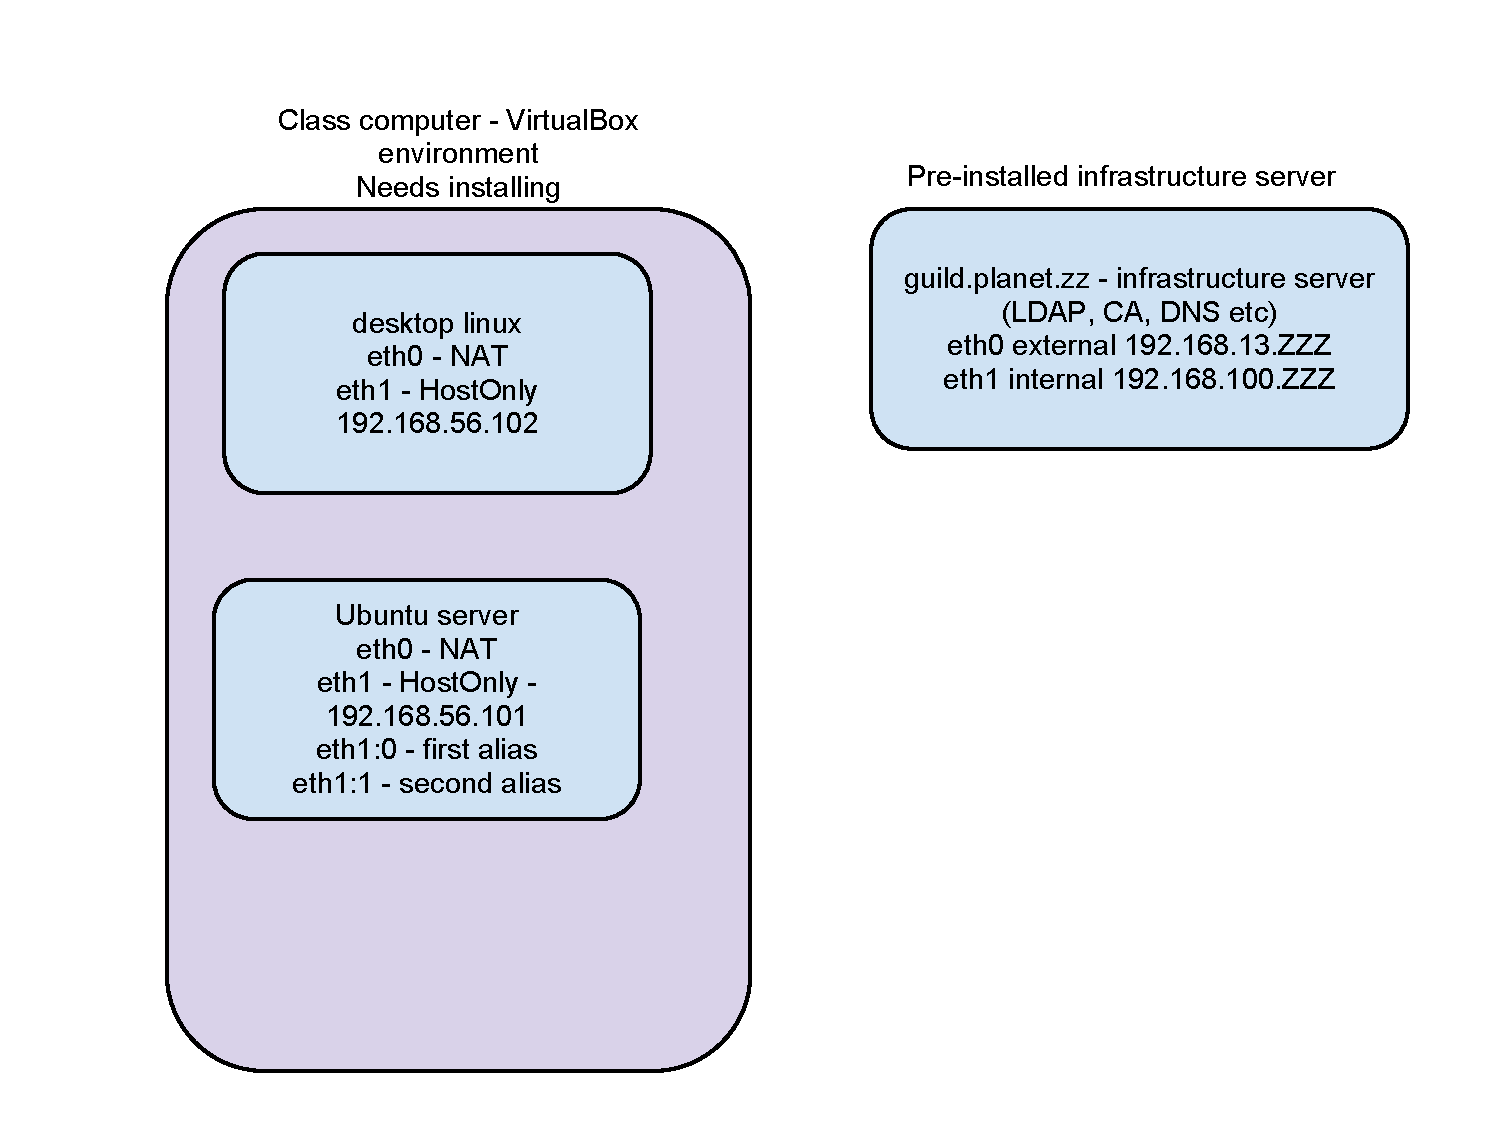
\includegraphics[width=\textwidth]{Lab_setup.pdf}
	\caption{Lab Setup}
	\label{Lab Setup}
\end{figure}



%Some unicode symbols
%道場

\begin{tikzpicture}
  \path[mindmap,concept color=black,text=white]
    node[concept] {Computer Science}
    [clockwise from=0]
    child[concept color=green!50!black] {
      node[concept] {practical}
      [clockwise from=90]
      child { node[concept] {algorithms} }
      child { node[concept] {data structures} }
      child { node[concept] {pro\-gramming languages} }
      child { node[concept] {software engineer\-ing} }
    }  
    child[concept color=blue] {
      node[concept] {applied}
      [clockwise from=-30]
      child { node[concept] {databases} }
      child { node[concept] {WWW} }
    }
    child[concept color=red] { node[concept] {technical} }
    child[concept color=orange] { node[concept] {theoretical} };
\end{tikzpicture}

\begin{tikzpicture}
  \path[mindmap,concept color=black,text=white]
    node[concept] {Course pre requirements skills}
    [clockwise from=0]
    child[concept color=green!50!black] {
      node[concept] {GNU/Linux}
      [clockwise from=90]
      child { node[concept] {Able to use text editor} }
      child { node[concept] {Understanding of File System Hierarchy} }
      child { node[concept] {pro\-gramming languages} }
      child { node[concept] {software engineer\-ing} }
    }  
    child[concept color=blue] {
      node[concept] {Experience with command line}
      [clockwise from=-30]
      child { node[concept] {file manipulation with cp,mv,touch,rm,mkdir etc} }
      child { node[concept] {user management with adduser, passwd, id, getent, usermod, addgroup, useradd, groupadd} }
    }
    child[concept color=red] { node[concept] {technical} }
    child[concept color=orange] { node[concept] {theoretical} };
\end{tikzpicture}





{\color{red} UURIDA analüüsiks

\url{jclarkgardner.com} - ilus tekst + VÄGA HEAD VIDEOD, kahjuks pole viidatav
\url{http://georgejoeckel.blogspot.com/}

\url{http://www.regent.edu/admin/ctl/coursedesign/home.cfm} - NB VAJA UURIDA

\url{http://www.instructionaldesign.org/models/addie_weaknesses.html} Weaknesses of the ADDIE Model
\url{http://www.learningsolutionsmag.com/articles/1012/}

\url{http://rjh.goingeast.ca/2011/07/05/design-research-for-online-learning-course-design-edumooc/} - uurida
}

Veel viiteid uurida 
{\scriptsize
\\

The Fog of Cyber Defence - \url{http://urn.fi/URN:ISBN:978-951-25-2431-0}

\url{http://www.emergencymgmt.com/safety/4-Priorities-Improving-Cybersecurity-US.html}\\
\url{http://www.umuc.edu/grad/gradprograms/csec.cfm}
\\
\url{http://www.poly.edu/academics/programs/cybersecurity-ms/curriculum}\\
\url{http://cms.montgomerycollege.edu/EDU/Plain.aspx?id=13043}\\
\url{http://cybersecurity.byu.edu/}\\
\url{http://gcn.com/articles/2010/07/09/cyber-command-panel-afcea-symposium.aspx}\\
\url{http://www.emergencymgmt.com/training/Cybersecurity-Curriculum-University-Maryland-Students.html}\\
\url{http://www.qatar.cmu.edu/iliano/courses/12F-CMU-CS349/index.php?page=info}\\
{\color{red} Analüüsi peatüki kirjutamiseks vaja uurida:}
http://www.commonexploits.com/?p=789
\url{http://www.tandfonline.com/} - UT võrgust kättesaadav! teadusajakirjad.
meterpreter scripts \url{http://www.offensive-security.com/metasploit-unleashed/Writing_Meterpreter_Scripts}
}


\section{Mõtteid, mida töös kasutada}

\begin{itemize}
\item Miks ei kaasata malware laborit? - Sysadminnid ei hakka malware analüüsima ja kasutavad virustotal abi + kohapeal paigaldatud antiviiruseid. Kuna need on põhiliselt tootjapõhised ja seda sorti asju siin ei kasutata (vaata nõuet XXX)
\end{itemize}




\chapter{Toormaterjal}
{\color{red} See ei ole osa tööst vaid asjad, mis jäävad tõenäoliselt välja}


Siin on asjad, kust tõstan mingid lõigud töösse

\begin{verbatim}
8.8.8.8; pwd

8.8.8.8; cp ../../config/config.inc.php /tmp/asi.txt

8.8.8.8; cat /tmp/asi.txt

Kuigi ping tulemuste all pole config faili sisu näha, 
tehes lehel parema kliki ja valides "View Page Source" näeme, et source faili sees on config.inc.php sisu olemas.


    DVWAs kasutades "Command execution" andmebaasi loomine:
    8.8.8.8; mysql --user=root --password='student' -e 'create database kala;'

Software eggs
http://www.itcollege.ee/?=PHPB8B5F2A0-3C92-11d3-A3A9-4C7B08C10000
    

\end{verbatim}

\url{http://blog.spiderlabs.com/2011/01/detecting-malice-with-modsecurity-csrf-attacks.html}

Lisada upstart ülesanne mysql oom score tuunimiseks.


DHCP laborisse lisada shared-network konfig

Iga peatüki juurde panna kirja, mitu lehekülge on vaja.
E-kiri tsitaatidena - ainult vajalikud osad.
ainekava ei tõlgi - Jääb lisasse eesti keelsena
neljapäeva hommikul 16. saadan töö. - tühja kohta ei ole - todo on tehtud ja jääb keelekorrektuur.
neljapäevaks kaitsmisproov.

 Todays studi in \gls{EITC} include lectures, practical classes and independent work as homework. By and large, one subject is divided as follows: 25\% lectures, 25\% practical classes and 50\% homework which is mostly working with materials (books, web articles). In the worst case, practical work constitutes only 25\% and takes place at \gls{EITC} computer classes.
Moreover, the students are not interested in learning mere theory. The formulas are not seen necessary nor linked to their study area or future job. Theory that is not used will be forgotten quickly. In a few years students won't even remember if a specific topic was covered or not. Applied education should introduce practical approach and learning by doing. In ITC field practical classes and practical homework is the key to achieving acceptable results.
In initial investigation phase the authors role was curricula development, requirements management,  planning hands-on labs and course descriptions.

{\color{red} 
Usable to design a learner centric course instead of teacher centric. 

\url{http://www.youtube.com/watch?v=zB92UMyYzKM}

Course content - get attencion
Ingeraction amoungs students
Jugement 
Student diversity - ebaühtlus
Create a role played scenario
Analyse the material.

\url{http://www.youtube.com/watch?v=oRgLqEF-qAU}

}

Serdi sees url -  Online Certificate Status Protocol (OCSP)
Saab teha ajaaknaga harjutusi. Teenuste uuendamine ja uure vahendite kasutamine ründamiseks...Kõik oleks ajas muutuv.

\url{http://www.createdebate.com/debate/show/How_relevant_is_the_ADDIE_model_in_2009}

ADDIE model \url{http://www.youtube.com/watch?v=fdpHO1xycgo&list=PLEBAA915299F438EB}


Haridustehnoloogia sõnastik - \url{http://wiki.e-uni.ee/htsonastik/index.php?n=Main.Otilde#oppematerjal}

Miks creative common - \url{http://www.copyrightreform.eu/case-for-copyright-reform}

Alternative Training Models
Advances in Developing Human Resources November 2006 8: 460-475,
Today a learning by doing approach is accepted way to gain new skills and knowledge in cyber security field. This thesis focuses to develop of the practical hands-on e-course for system administrators in \gls{EITC}. Moreover the developed laboratories are used in higher education and also in continuous education classes.
